% XXX Jedes Jahr Mensa-Preise prüfen!
\section[Das kleine Mensa~1~×~1]{\boldmath Das kleine Mensa~${1 \times 1}$}
\begin{multicols*}{2}
\begin{quote}
	\textit{Allein zu essen ist für einen philosophierenden Gelehrten ungesund.}
	
	\hfill--- Immanuel Kant
\end{quote}

Alltäglich gegen Mittag beginnt der Magen zu knurren.
Für die Leute, die nicht jeden Tag nach Hause fahren oder selber kochen können -- also wenn Mutti zu weit weg wohnt -- gibt es die Mensa.
Das Gute ist, dass die Mensa~am~Ring (ehemals Mensa~II) direkt nebenan liegt.
Die meisten Studierenden gehen um 12~Uhr direkt in die Mensa.

Dort erwartet euch zunächst eine große Schlange, denn um 12~Uhr ist der Anlauf dort am größten (die älteren Semester versuchen es daher eine Viertelstunde früher einzurichten).
Doch diese Schlange ist meist nach kurzer Zeit überraschenderweise überwunden.
Bevor man sich anstellt, sollte man allerdings so einiges über die Mensa wissen!

Seit dem Sommersemester 2017 benötigt man zum Bezahlen lediglich seinen Studierendenausweis.
Das Guthaben darauf kann an den Automaten im Foyer der Mensa aufgeladen werden.
Wenn das Guthaben nicht mehr ausreicht um euer Essen zu bezahlen, könnt ihr das Guthaben auch an der Kasse noch aufladen. 
Das ist jedoch mit einem kleinen Aufpreis behaftet und die Missgunst der Kassiererin, sowie aller die in der Schlange hinter euch stehen ist euch sicher.
Falls ihr den Studierendenausweis noch nicht zugeschickt bekommen habt, könnte das daran liegen, dass ihr noch kein Foto dafür hochgeladen habt.
Das solltet ihr dann so bald wie möglich nachholen.

\begin{center}
	\includegraphics[width=\columnwidth]{private/res/studierendenausweis.pdf}
\end{center}

Falls ihr diese Hürde geschafft habt, stellt sich jeden Mittag erneut die Frage, was es überhaupt zu Essen gibt und was du selbst essen willst.
Dazu gibt es einmal den Mensaplan, der an der Information ausliegt und auch in ein paar Werbeblättern wie der "na dann\dots" (welche in der Mensa auch meist in irgendeiner unscheinbaren Ecke ausliegt) abgedruckt ist.
Diesen Mensaplan könnt ihr auch auf der Website der Mensa

(Link: \url{https://www.stw-muenster.de/de/essen-trinken/mensen/am_ring})

einsehen oder euch wöchentlich als Newsletter per E-Mail zuschicken lassen.
Es gibt auch die Mensa-App (für Android-Geräte im Google~Play Store, für iPhones im App-Store).
Doch dieser Mensaplan beinhaltet nur die Menus, welche in der oberen Essensausgabe ("Oben") angeboten werden.
Auf den großen LCD-Bildschirmen im Foyer der Mensa könnt ihr jedoch alle Tagesangebote (z.\,B.\ auch die Beilagen und Desserts) und Preise erfahren.
Hier stehen auch die Angebote des Buffetsaals ("Unten").

"Oben" werden immer 3~Menüs angeboten, welche mit einem malerischen Namen gekennzeichnet sind (z.\,B.\ "Schnitzel Hubertus-Art" für ein scheinbar frittiertes Schnitzel mit Pilzsauce).
Preislich liegen die Menüs bei \SIlist{2,30; 2,95; 3,30}{\euro} und beinhalten drei mehr oder minder passende Beilagen.
Jede weitere Beilage liegt bei \SI{0,25}{\euro}; lasst ihr eine Beilage weg, bedeutet das einen Nachlass von ebenfalls \SI{0,25}{\euro}.
Solltet ihr jedoch kein Menü haben, so liegt die Beilage bei \SI{0,65}{\euro}.
Abhilfe schaffen hier meistens der Satz "Ich hatte schon ein Menü" oder die Bezahlung durch einen Kommilitonen mit Menü.
Die Glasschälchen mit ausgefalleneren Desserts sind für \SI{0,95}{\euro} zu haben.
Täglich ist mindestens ein Menü vegetarisch.
Zusätzlich gibt es eine vegane Theke mit einem Gericht und dem veganen Salatbuffet.
Dort gibt es auch einen Beilagensalat, der verlässlich nicht mit dem eher unbeliebten Joghurtdressing versehen ist.

Die häufigen Mensabesucher werden jedoch schnell bemerken, dass die Menüauswahl sich alle 4--6~Wochen wiederholt.
Das ist aber gar nicht so schlimm, denn die Menüs schmecken dann wieder genauso gut oder schlecht wie zuvor; so bildet sich langsam ein kompetenter Mensabesucher aus dir heraus.
Bei den ersten Besuchen solltet ihr aufpassen, dass die Bilder auf den Bildschirmen oftmals nicht im Entferntesten mit dem Aussehen des Essens übereinstimmen.

\begin{center}
	\fibelimgtext[bottom left]{
		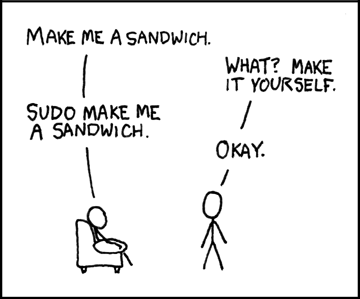
\includegraphics[width=0.95\columnwidth]{res/xkcd/149_sandwich.png}
	}{\url{https://xkcd.com/149}}
\end{center}

"Unten" gibt es ein vielfältiges Angebot von immer wiederkehrenden Menüs.
Jeden Tag könnt ihr an der Grillstation Currywurst mit Pommes oder ein Jäger-/Zigeunerschnitzel erwerben.
Montags gibt es den beliebten Mensaburger (auch vegetarisch), welcher so groß ist, dass sich an ihm die Geister scheiden, ob er mit Messer und Gabel oder mit der Hand gegessen werden muss.
Im Winter wird an der Eintopfstation oft ein preiswerter Eintopf angeboten.
Falls ihr Pommes nehmt, ist es empfohlen, mit Pommessalz nachzusalzen und gegen einen kleinen Aufpreis Majo oder Ketchup zu erstehen.
Senf dagegen ist wie in einer richtigen Frittenbude kostenlos.
Das Beste am Buffetsaal sind in meinen Augen jedoch die abwechselnden und wiederkehrenden Tagesmenüs.
So wundert euch nicht am Donnerstag über die große Schlange, denn es gibt dann immer das allseits beliebte Gyros mit Zaziki und Pommes, welches sich auch ideal als Katerfrühstück eignet.
Dazu noch eine Cola und manche Leute sind etwa 4~Euro und ihren donnerstags wegen der tollen Mittwochsaktionen in Eule, AMP, Schaf und Co.\ erstandenen Kater los.


\includegraphics[width=\columnwidth]{res/muenster_isst_veggie.png}

Des Weiteren gibt es unter dem Motto "Münster isst veggie" am Donnerstag ein weiteres vegetarisches Menü.
An anderen Tagen gibt es im Buffetsaal auch Wraps, Pizza oder saisonal Grünkohl- oder Spargelmenüs.
Ein weiterer Pluspunkt des Buffetsaals ist jedoch die Salattheke.
Hier könnt ihr euch mit vielen verschiedenen Salatsorten euren eigenen Salat kreieren und klassisch mit (Balsamico-)Essig und Öl oder mit einem Joghurt- oder Cocktaildressing garnieren.
Dazu könnt ihr ein Baguettebrötchen oder auch ein paar Nudelsorten und Saucen oder übriggebliebene Aufläufe vom Vortag wählen.
Das Ganze kostet dann \SI{0,57}{\euro} pro \SI{100}{\g}.
Zu jedem Essen gibt es ein recht gut sortiertes Angebot an preiswerten Getränken.

Wenn ihr fertig mit dem Essen seid, seid ihr noch lange nicht mit der Mensa fertig!
Entweder ihr holt euch noch einen Nachschlag ("Ich hatte schon ein Menü") oder ihr macht euch mit eurem Tablett auf zum Geschirrband und der meist etwas murrig schauenden Person dort.
An der Wand hängt dann eine genaue Anleitung, wie ihr euer Geschirr zu sortieren habt, damit es keinen Ärger vom Mensapersonal gibt.

\fibelimgtext{
	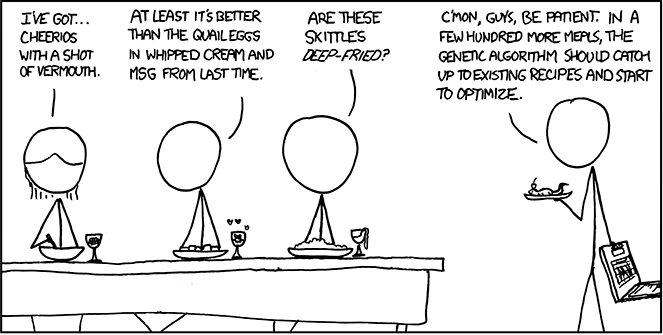
\includegraphics[width=\columnwidth]{res/xkcd/720_recipes.png}
}{\url{https://xkcd.com/720}}

Falls jedoch jemand gar nichts gefunden haben sollte, kann er es auch mit einem Brötchen oder Rühr- oder Spiegelei im Café Viva versuchen.
Hier werden auch die meisten anstehenden Sportereignisse übertragen und morgens in der Wiederholung gezeigt.
Außerdem kann man hier recht entspannt sitzen und mit mehreren eine Kaffeespezialität trinken.

Im Foyer sind außerdem noch ein kleiner Kiosk mit Getränken und Süßigkeiten und ein Eismann, welcher im Winter auch leckere Waffeln anbietet.

Dazu kommen noch diverse Läden wie ein Copyshop (mit etwas gehobenen Preisen!
Es ist preiswerter, Print~\&~Pay beim ZIV einzurichten oder -- solltet ihr im Besitz einer Mensacard sein -- an den Kopierern, z.\,B.\ in der AP-Bibliothek, der IG1 oder im ZIV, zu kopieren.
Aber vergesst eure Karte dort nicht!), eine Filiale der Techniker-Krankenkasse und der Aster-Reiseservice.

Alternativ könnt ihr auch die anderen Mensen in Münster besuchen, insbesondere die größte, die Mensa~am~Aasee (ehemals Mensa~I), sei hier aufgrund der großen Auswahl an Salaten und dem grandiosen Buffet am Abend empfohlen.

\fibelsig{Friedrich}
\end{multicols*}
